\documentclass[a4paper,14pt]{extreport}
\usepackage[left=1.5cm,right=1.5cm,
    top=1.5cm,bottom=2cm,bindingoffset=0cm]{geometry}
\usepackage{scrextend}
\usepackage[T1,T2A]{fontenc}
\usepackage[utf8]{inputenc}
\usepackage[english,russian,ukrainian]{babel}
\usepackage{tabularx}
\usepackage{amssymb}
\usepackage{color}
\usepackage{amsmath}
\usepackage{mathrsfs}
\usepackage{listings}
\usepackage{graphicx}
\graphicspath{ {./images/} }
\usepackage{lipsum}
\usepackage{xcolor}
\usepackage{hyperref}
\usepackage{tcolorbox}
\usepackage{tikz}
\usepackage[framemethod=TikZ]{mdframed}
\usepackage{wrapfig,boxedminipage,lipsum}
\mdfdefinestyle{MyFrame}{%
linecolor=blue,outerlinewidth=2pt,roundcorner=20pt,innertopmargin=\baselineskip,innerbottommargin=\baselineskip,innerrightmargin=20pt,innerleftmargin=20pt,backgroundcolor=gray!50!white}
 \usepackage{csvsimple}
 \usepackage{supertabular}
\usepackage{pdflscape}
\usepackage{fancyvrb}
%\usepackage{comment}
\usepackage{array,tabularx}
\usepackage{colortbl}

\usepackage{varwidth}
\tcbuselibrary{skins}
\usepackage{fancybox}


\usepackage{tikz}
\usepackage[framemethod=TikZ]{mdframed}
\usepackage{xcolor}
\usetikzlibrary{calc}
\makeatletter
\newlength{\mylength}
\xdef\CircleFactor{1.1}
\setlength\mylength{\dimexpr\f@size pt}
\newsavebox{\mybox}
\newcommand*\circled[2][draw=blue]{\savebox\mybox{\vbox{\vphantom{WL1/}#1}}\setlength\mylength{\dimexpr\CircleFactor\dimexpr\ht\mybox+\dp\mybox\relax\relax}\tikzset{mystyle/.style={circle,#1,minimum height={\mylength}}}
\tikz[baseline=(char.base)]
\node[mystyle] (char) {#2};}
\makeatother

\definecolor{ggreen}{rgb}{0.4,1,0}
\definecolor{rred}{rgb}{1,0.1,0.1}
\definecolor{amber}{rgb}{1.0, 0.75, 0.0}
\definecolor{babyblue}{rgb}{0.54, 0.81, 0.94}
\definecolor{asparagus}{rgb}{0.53, 0.66, 0.42}
\definecolor{chartreuse}{rgb}{0.5, 1.0, 0.0}
\definecolor{darkorchid}{rgb}{0.6, 0.2, 0.8}
\definecolor{apricot}{rgb}{0.98, 0.81, 0.69}
\definecolor{bittersweet}{rgb}{1.0, 0.44, 0.37}
\definecolor{classicrose}{rgb}{0.98, 0.8, 0.91}

\usepackage{float}
\usepackage{wrapfig}
\usepackage{framed}
%for nice Code{
\lstdefinestyle{customc}{
  belowcaptionskip=1\baselineskip,
  breaklines=true,
  frame=L,
  xleftmargin=\parindent,
  language=C,
  showstringspaces=false,
  basicstyle=\small\ttfamily,
  keywordstyle=\bfseries\color{green!40!black},
  commentstyle=\itshape\color{purple!40!black},
  identifierstyle=\color{blue},
  stringstyle=\color{orange},
}
\lstset{escapechar=@,style=customc}
%}


\begin{document}
\pagecolor{white}

%----------------------------------------1
\newtcbox{\xmybox}[1][red]{on line, arc=7pt,colback=#1!10!white,colframe=#1!50!black, before upper={\rule[3pt] {0pt}{10pt}},boxrule=1pt,boxsep=0pt,left=6pt,right=6pt,top=2pt,bottom=2pt}

\begin{center}Лищенко Богдан  ДП-82
\vspace{1cm}
\end{center}


\begin{center}1\end{center}
Чим визначається квантовий стан вільного електрона?\\

Квантовий стан вільного електрона задається значенням його хвильового
числа k. або квазімпульсу $P = \hbar \cdot k $. Скільки таких квантових станів припадатиме вибраний скінченний інтервад енергії, залежатиме від вимірності системи, в якій перебуває слектрон, її протяжності, а також від аналітичної залежності між енергією електрона і його хвильовим числом, тобто від закону дисперсії.


\begin{center}2\end{center}
Дайте визначення густини станів вільного електрона.\\

Густина станів в 3D системах визначає об'ємну конпентрацію носіїв
зарялу, а її розмірність - об'єм. Густина станів в 2D системах визначає поверхневу концентрацію носіїв зарялу. Її розмірність - об'єм. Розмірність густини станів в 1D системах, де вона визначає лінійну
концентрацію носіїв заряду, об'єм.\\

Також знаючи об'єм простору, який припадає на один квантовий стан
вільного електрона у системі довільної вимірності, неважко розрахувати як
тустину станів вільних електронів, так і її енергетичну залежність. Для того, щоб це зробити, тобто щоб знайти кількість станів, які припадають на
одиничний інтервал енергій в околі енергії Е, потрібно знайти
"об'єм"\text{ } k-простору, який лежить між "поверхнями" \text{ } постійних енергій Е і Е+dE,
поділити його на об'єм k-простору, шо припалає на один квантовий стан,
врахувати двократне виродження за спіном і звести одержаний результат до
линичного інтервалу енергії, тобто поділити його на всличину приросту
енергії dЕ. Зрозуміло, що зазначений "об'єм" \text{ } буде власне об'ємом у
традиційному розумінні цього слова тільки для 3D систем. Для 2D систем він
насправді буде площею плоскої ділянки $k_x0k_y$, що лежить між лініями постійної енергії Е і Е+dE, а для 1D систем - протяжністю лінійної ділянки осі $0k_x$, що лежить між значеннями k, які відповідають єнергіям Е і Е+dE. Однак потрібно пам'ятати, що якщо об'єм. k-простору, який припалає на один квантовий стан електрона у будь-якій системі, визначається тільки і виключно її вимірністю і розмірами, то розподіл цих станів шкалою енергії, їхня густина принципово
будуть визначатися ще і законом дисперсії носіїв заряду Е(k). Останнє є
наслідком того, що густина станів нормується на одиничний інтервал єперітї, а який інтервал значень хвильових чисел відповідатиме одиничному інтервалу енергії вільних електронів, якраз і визначається аналітичною залежністю Е(k).

\begin{center}3\end{center} Сформулюйте і обгрунтуйте алгоритм розрахунку енергетичної залежності густини станів вільних електронів.
$$
S(k, E)=4 \pi k^{2}
$$

$$
V_{k}=S(k, E) d k(E)
$$
то згідно з законом диспсрсії
$$
\frac{d E}{d k}=\frac{\hbar^{2} k}{m}
$$

$$
d k=\frac{m}{\hbar^{2} k} d E
$$
тоді
$$
V_{k}=4 \pi k^{2} \frac{m}{h^{2} k} d E=\frac{4 \pi m}{h^{2}} k d E
$$

$$
k=\frac{\sqrt{2 m E}}{h}
$$

Кількість станів в енергетичному інтервалі dE на рівні Е у системі розмірів $L$ вbзначається як густина станів $\rho_{L}(E)$, помножена на величину енергетичного інтервалу $d E$. Oтжe,
$$
\rho_{L}(E) d E=\frac{V_{k}}{V_{1}} \cdot 2=L^{3} \frac{(2 m)^{3 / 2}}{2 \pi^{2} \hbar^{3}} \sqrt{E} d E
$$
Двійка в останньому співвідношенні враховує двократнс виролження квантових станів слектрона за спіном. Скоротнвши праву і ліву частини на $d E$, одержуємо
$$
\rho_{L}(E)=L^{3} \frac{(2 m)^{3 / 2}}{2 \pi^{2} \hbar^{3}} \sqrt{E}
$$
Дия системи одиничних розмірів ( $L=1)$
$$
\rho(E)=\frac{(2 m)^{3 / 2}}{2 \pi^{2} \hbar^{3}} \sqrt{E}
$$
Густина сганів в $3 D$ системах визначае об'ємну коннентранію носії 3apsuy, a iї posmipriorb $-e B^{\prime}$

З останнього співвідношення випливає, шо у тривимірних системах густина
станів вільних електронів є степенсвою функцією ефективної маси носіїв зарялу та їхньої снергії і зростає зі збільшенням останніх за законом ро - $\rho \approx m^{3/2}E^{1/2}$


\begin{center}4\end{center}
Охарактеризуйте закономірності модифікації енергетичної залежності густини станів вільних носіїв зарядів у разі зміни вимірності структури у системах з фіксованим законом дисперсії.\\


\begin{center}5\end{center}
Покажіть залежність густини станів вільного електрона від його ефективної маси і обгрунтуйте фізичні засади і причини такої залежності;\\

Для системи одиничних розмірів $(L=1)$
$$
\rho(E)=\frac{(2 m)^{3 / 2}}{2 \pi^{2} \hbar^{3}} \sqrt{E}
$$
Густина станів в $3 D$ системах визначае об'ємну концентрапію носіїв
3 попереднього співвідношення  випливає, шо у тривимірних снстемах rycтина станів вільних електронів є степеневою функщією ефективної маси носії заряду та іхньої енсргії і зростає зі збільшенням останніх за законом $\rho - m^{3 / 2} E^{1 / 2}$.

\begin{center}6\end{center}
Поясніть специфіку формування повної густини станів  систем з вільними 2D електронами з урахуванням великої кількості двовимірних енергетичних  зон.\\

\begin{figure}[h]
\center{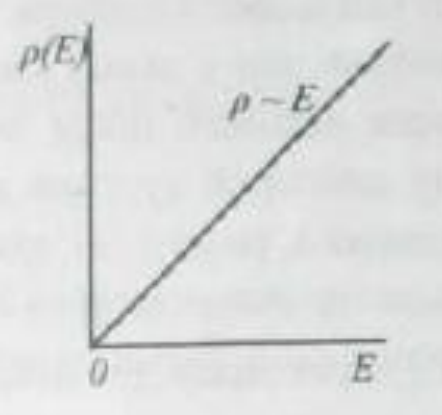
\includegraphics[width=0.2\linewidth]{1.png}}
\label{ris1}
\end{figure}
k-простору, що лежить між колами постійної енергії $E$ і $E+d E$, становитиме
$$
S_{k}=\frac{2 \pi \alpha^{2}}{h^{2}} E d E
$$
що дає такий вираз для густини станів:
$$
\rho(E)=\frac{\alpha^{2} E}{\pi h^{2}}
$$
Густина станів $2 D$ електронів з лінійним законом дисперсії лінійно
на рис.\ref{ris1} .


\begin{center}7\end{center}
Зобразіть графічно залежність густини станів вільного електрона від енергії для систем різної вимірності  з різними законами дисперсії з урахуванням великої кількості енергетичних зон розмірного квантування.

\end{document}
